\documentclass[tikz,border=8pt]{standalone}
\begin{document}
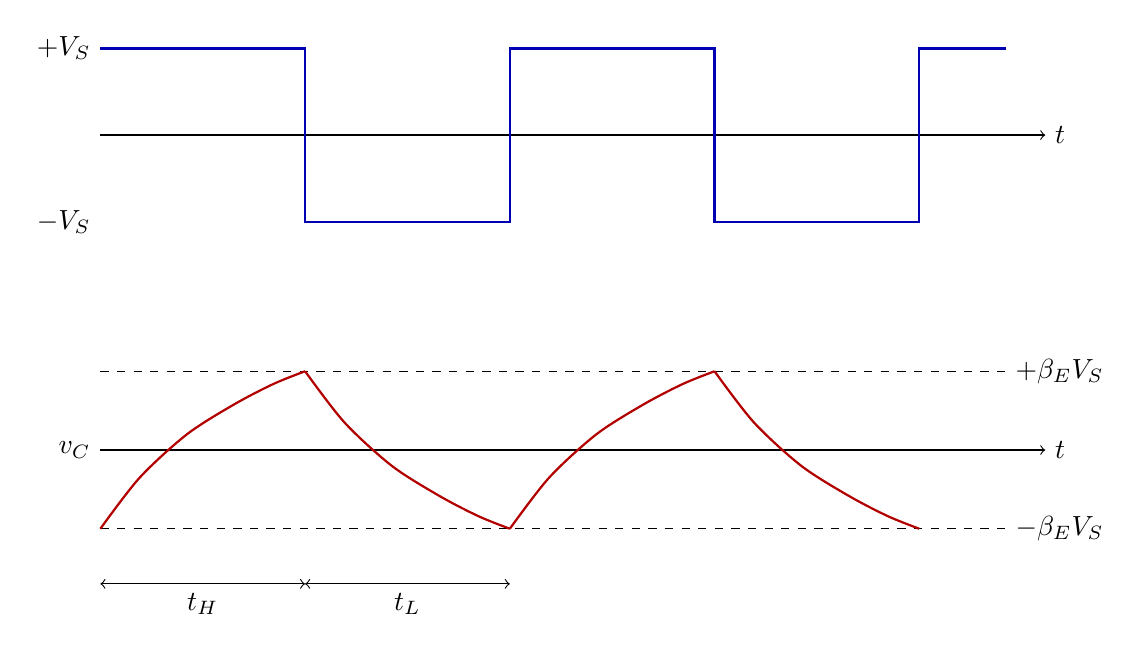
\begin{tikzpicture}[font=\sffamily,x=1cm,y=1cm]
\draw[->] (0,0)--(12,0) node[right]{$t$};
\draw[blue!70!black,thick] (0,1.1)--(2.6,1.1)--(2.6,-1.1)--(5.2,-1.1)--(5.2,1.1)--(7.8,1.1)--(7.8,-1.1)--(10.4,-1.1)--(10.4,1.1)--(11.5,1.1);
\node[left] at (0,1.1) {$+V_S$}; \node[left] at (0,-1.1) {$-V_S$};
\draw[->] (0,-4)--(12,-4) node[right]{$t$};
\draw[dashed] (0,-3)--(11.5,-3) node[right]{$+\beta_E V_S$};
\draw[dashed] (0,-5)--(11.5,-5) node[right]{$-\beta_E V_S$};
\draw[red!70!black,thick] plot[smooth] coordinates {(0,-5)(.5,-4.35)(1.1,-3.8)(1.7,-3.42)(2.2,-3.16)(2.6,-3)};
\draw[red!70!black,thick] plot[smooth] coordinates {(2.6,-3)(3.1,-3.65)(3.7,-4.2)(4.3,-4.58)(4.8,-4.84)(5.2,-5)};
\draw[red!70!black,thick] plot[smooth] coordinates {(5.2,-5)(5.7,-4.35)(6.3,-3.8)(6.9,-3.42)(7.4,-3.16)(7.8,-3)};
\draw[red!70!black,thick] plot[smooth] coordinates {(7.8,-3)(8.3,-3.65)(8.9,-4.2)(9.5,-4.58)(10,-4.84)(10.4,-5)};
\draw[<->] (0,-5.7)--(2.6,-5.7) node[midway,below]{$t_H$};
\draw[<->] (2.6,-5.7)--(5.2,-5.7) node[midway,below]{$t_L$};
\node[left] at (0,-4) {$v_C$};
\end{tikzpicture}
\end{document}
